\documentclass{article}
\usepackage{tikz, comment}
\usepackage{pifont}
\usepackage{fontspec, pgfplots}
\usetikzlibrary{arrows, decorations.markings, decorations.pathreplacing}
\begin{comment}
:Title: Not defined yet
:Tags: moment;point of division formula;circumcenter;point of symmetry;focus of a parabola
:Prob: 0.4703;0.4648;0.4609;0.4516;0.4459
:Author: Prof.Hu Ji-shan, HKUST
:Slug: No name yet

Description Here.........
\end{comment}
\begin{document}\centering 

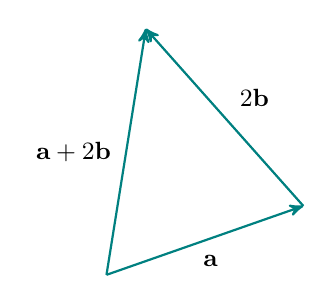
\begin{tikzpicture}[>=latex,xscale=.5*5, yscale=.5*5][font=\sf\small] 

\draw[teal, thick, ->, >=stealth'] (0, 0) -- (1, 0.35)node[black, below, midway, pos=0.5, xshift=2, yshift=-2, scale=1]{$\bf a$}; %a

\begin{scope}[xshift=1cm,yshift=0.35cm]
\draw[teal, thick, ->, >=stealth'] (0, 0) -- ({-0.4*2}, {0.45*2})node[black, right, midway, pos=0.5, xshift=2, yshift=7, scale=1]{$2\bf b$}; %2b

\end{scope}

\draw[teal, thick, ->, >=stealth'] (0, 0) -- ({1-0.4*2}, {0.35+0.45*2})node[black, left, midway, pos=0.5, xshift=-2, yshift=0, scale=1]{${\bf a} + 2\bf b$}; %a+2b

\end{tikzpicture}
\end{document}